\section{GPS-tracks}

Geo-tracks represent ...

\begin{figure}[!htp]
\centering
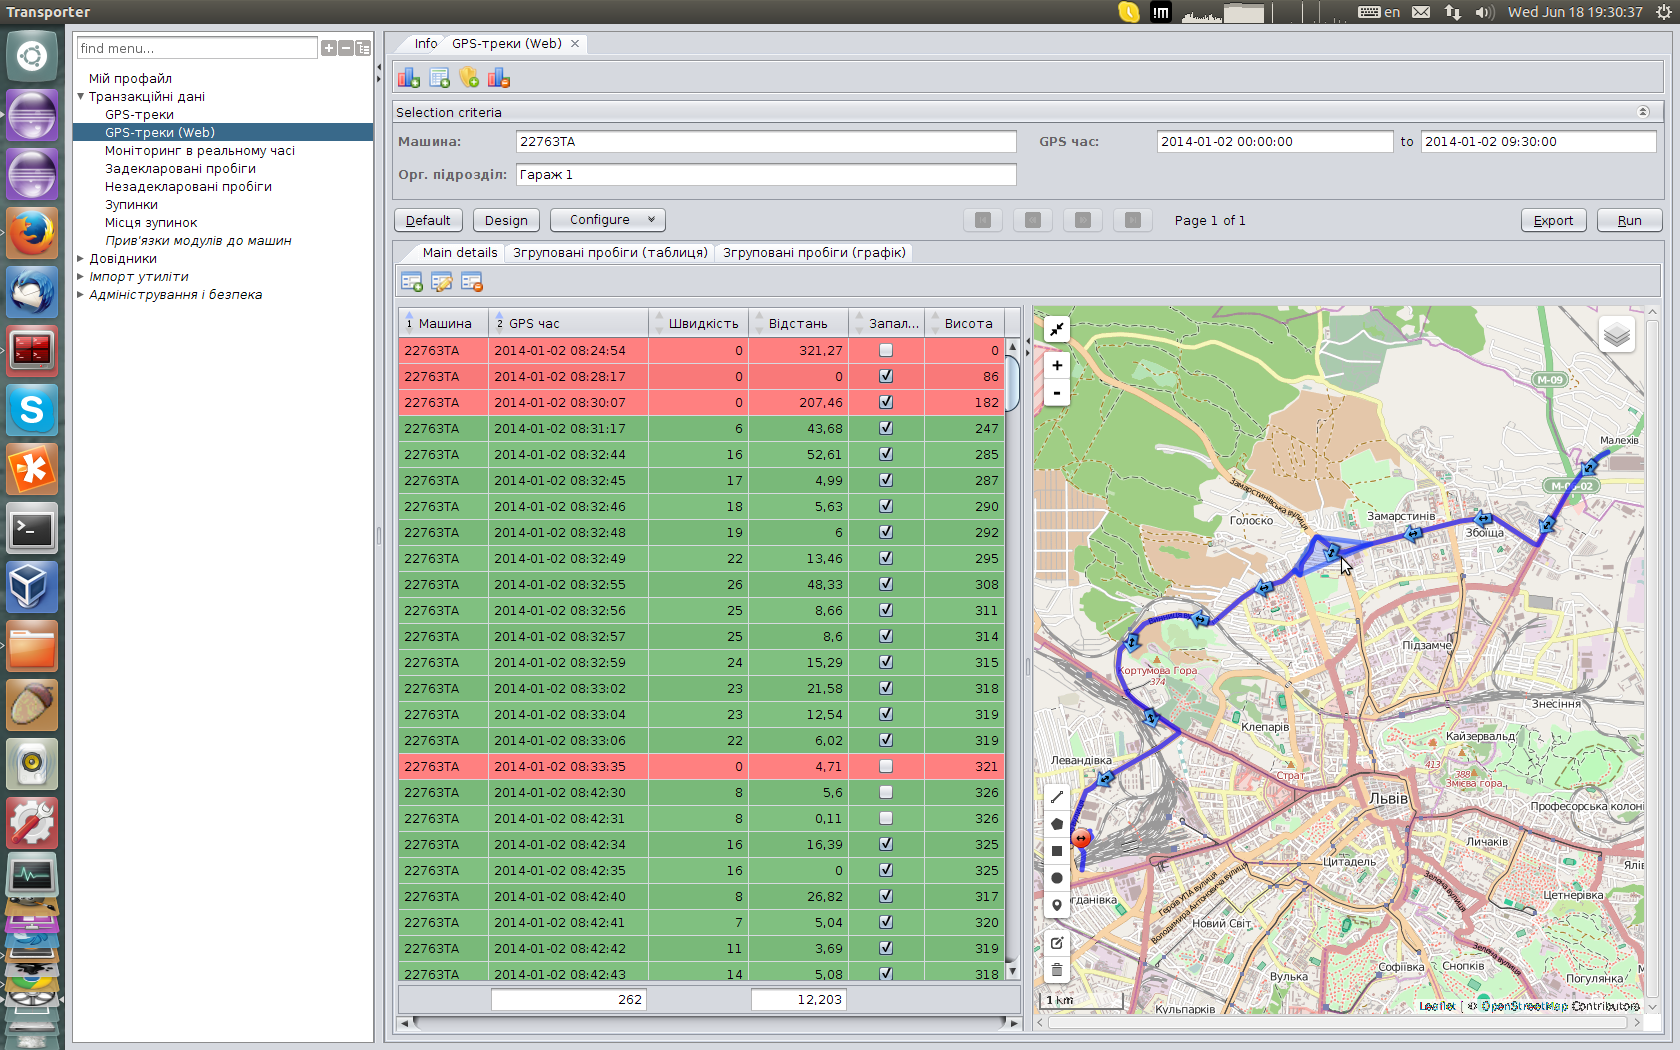
\includegraphics[width=16cm]{chapters/02-gpstracks/images/11-clusterised-gps-track-view-with-hovered-cluster.png}
\caption{clusterised-gps-track-view-with-hovered-cluster}\label{fig:11}
\end{figure}

\begin{figure}[!htp]
\centering
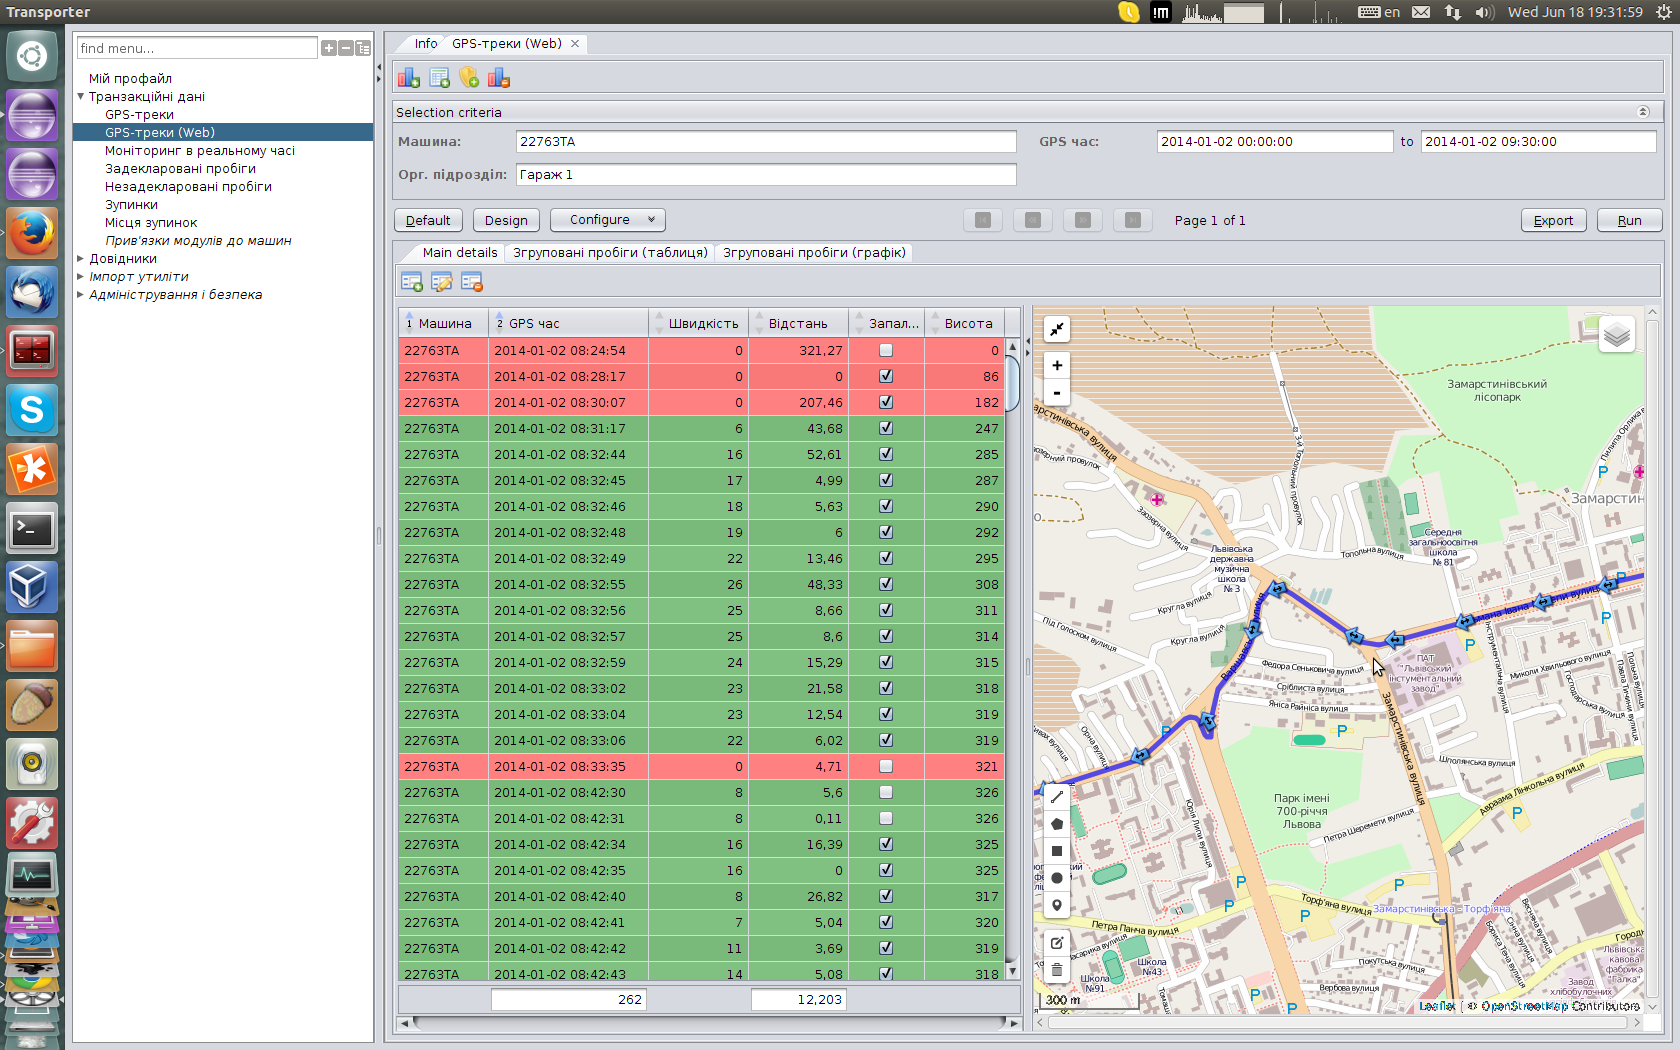
\includegraphics[width=16cm]{chapters/02-gpstracks/images/12-zooming-by-clicking-a-cluster.png}
\caption{zooming-by-clicking-a-cluster}\label{fig:12}
\end{figure}

\begin{figure}[!htp]
\centering
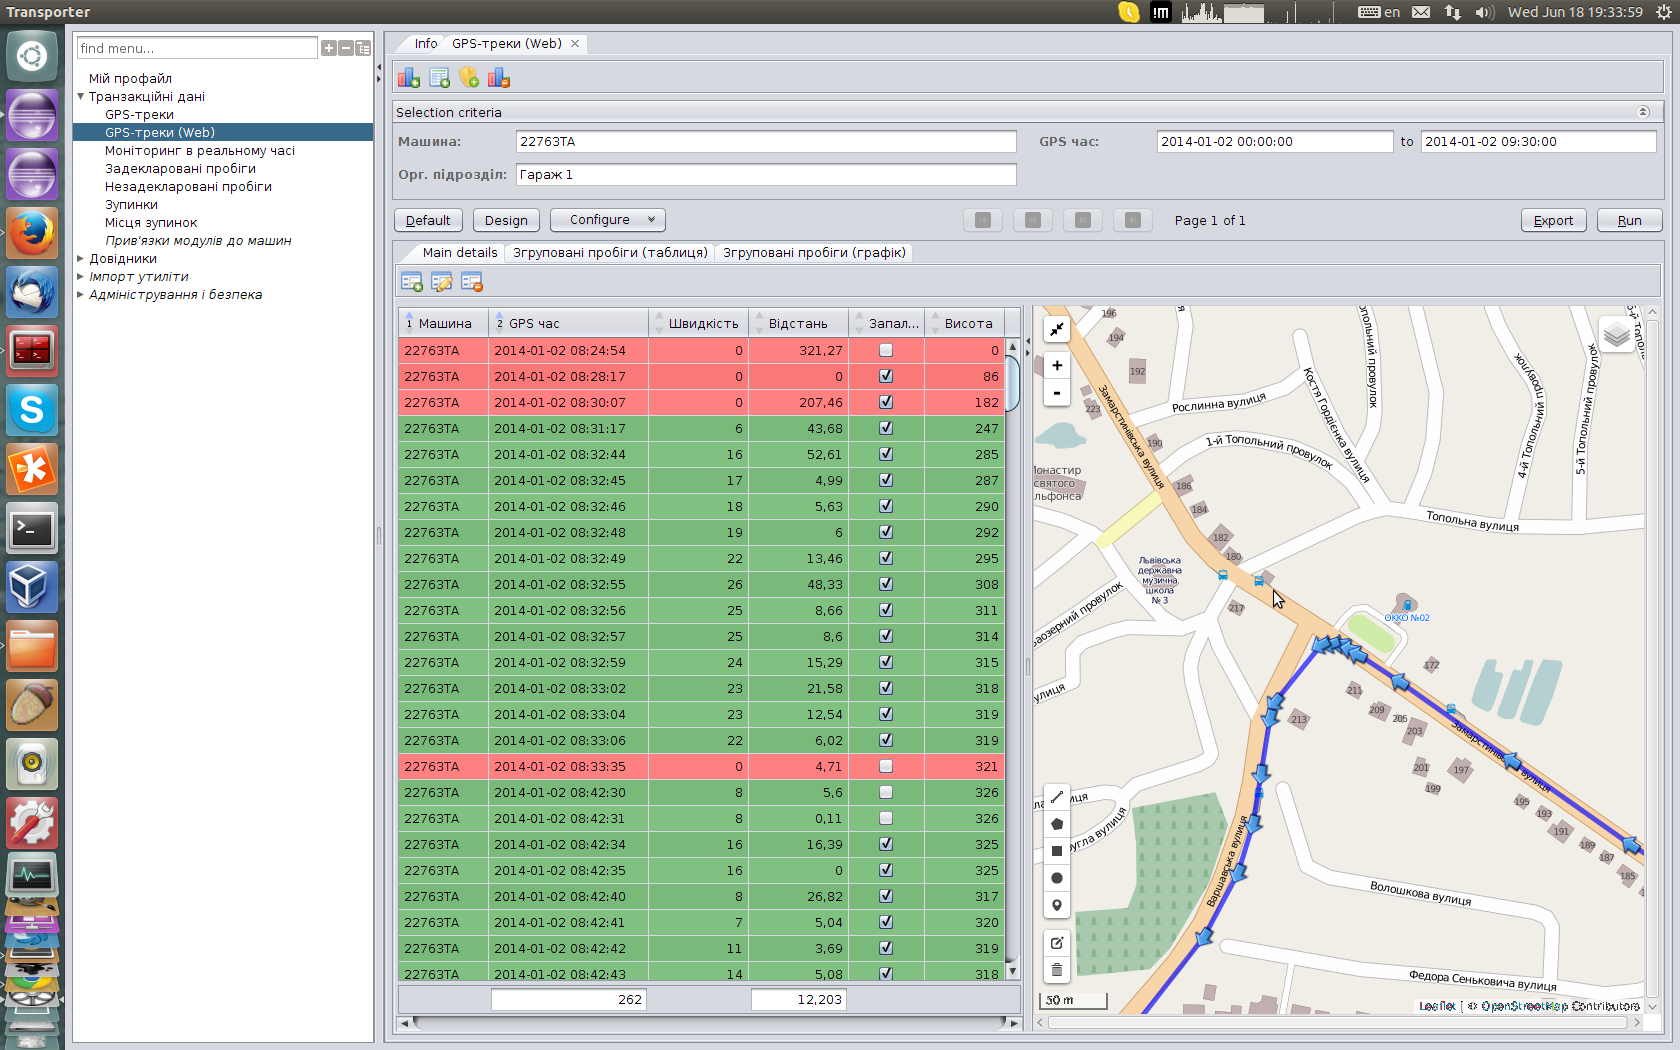
\includegraphics[width=16cm]{chapters/02-gpstracks/images/13-detailed-gps-track-view.png}
\caption{detailed-gps-track-view}\label{fig:13}
\end{figure}

\begin{figure}[!htp]
\centering
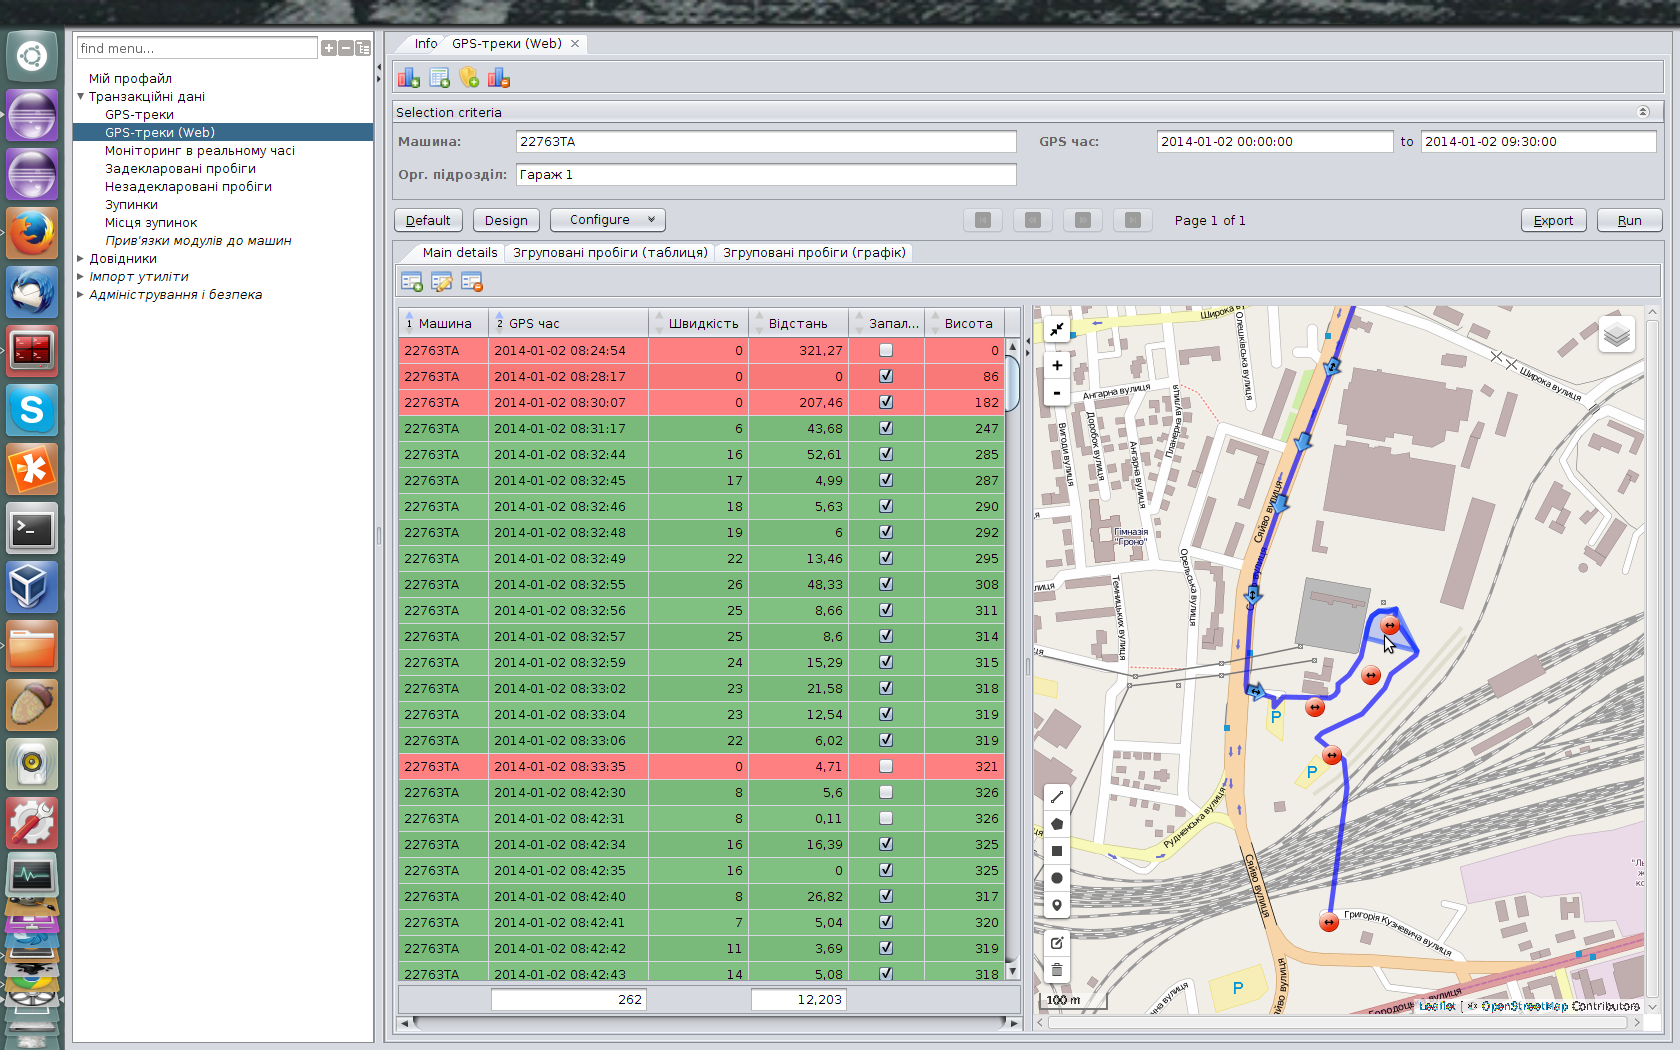
\includegraphics[width=16cm]{chapters/02-gpstracks/images/14-clusters-with-stoppage-messages-with-zero-speed.png}
\caption{14-clusters-with-stoppage-messages-with-zero-speed}\label{fig:14}
\end{figure}

\begin{figure}[!htp]
\centering
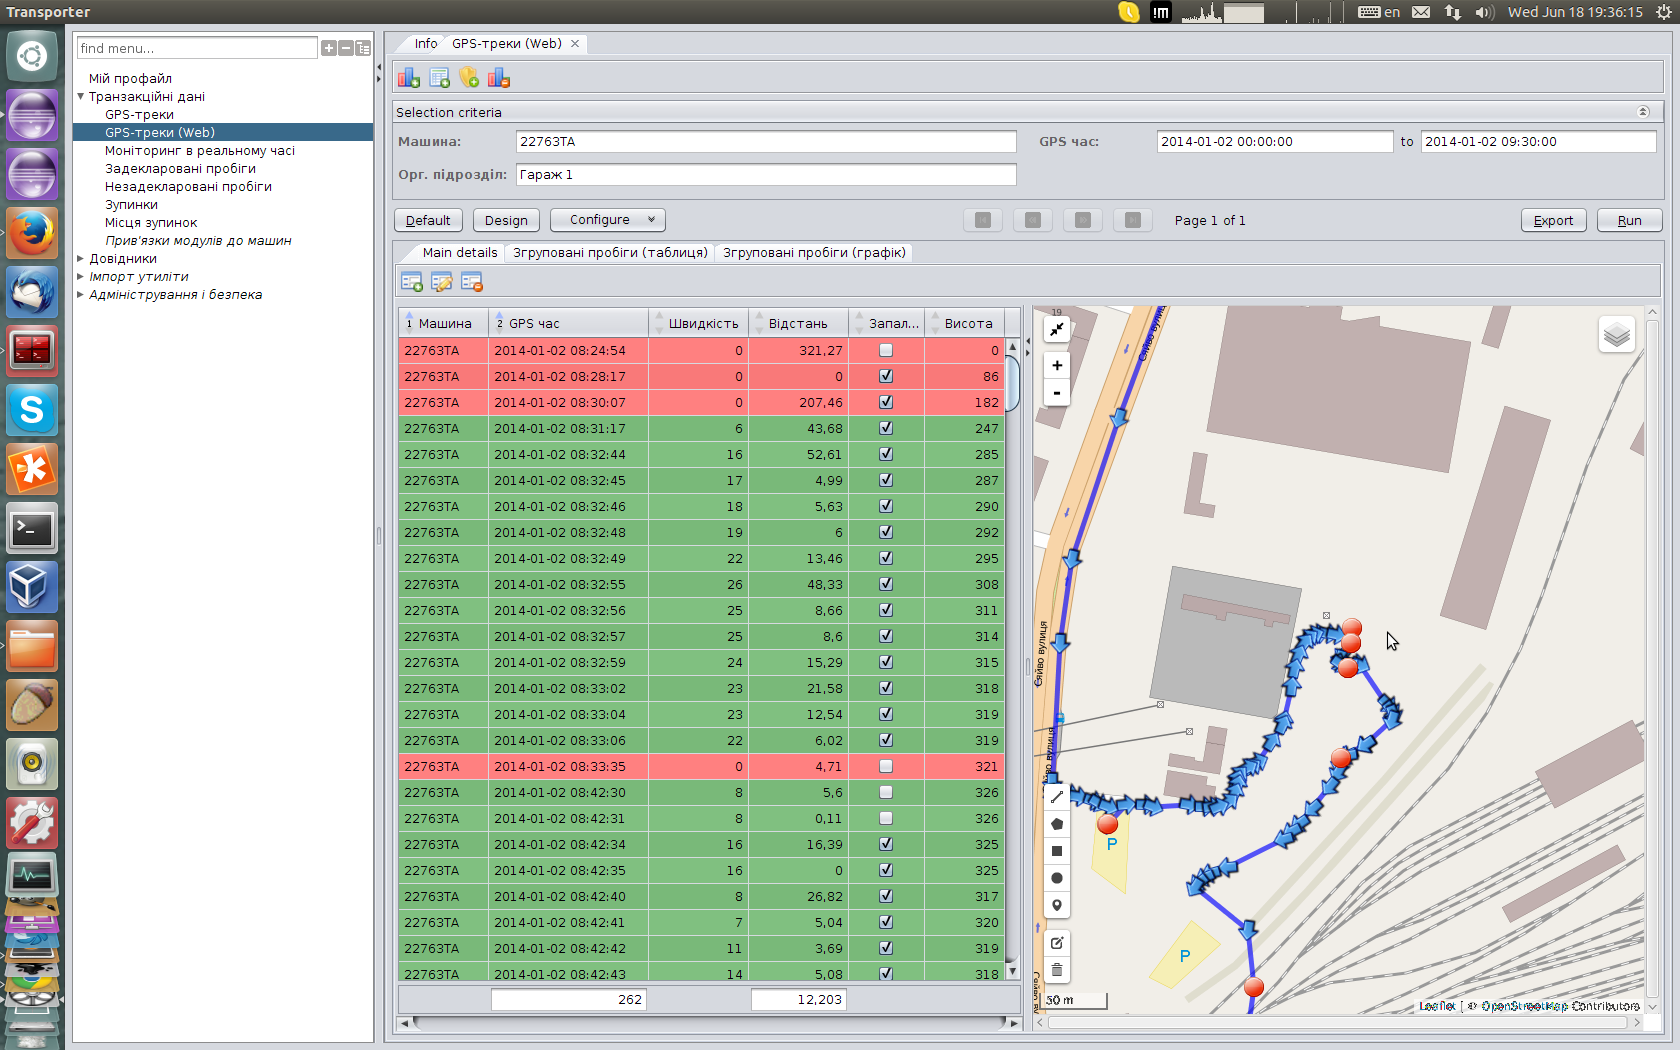
\includegraphics[width=16cm]{chapters/02-gpstracks/images/15-detailed-view-with-stoppages.png}
\caption{detailed-view-with-stoppages}\label{fig:15}
\end{figure}

\begin{figure}[!htp]
\centering
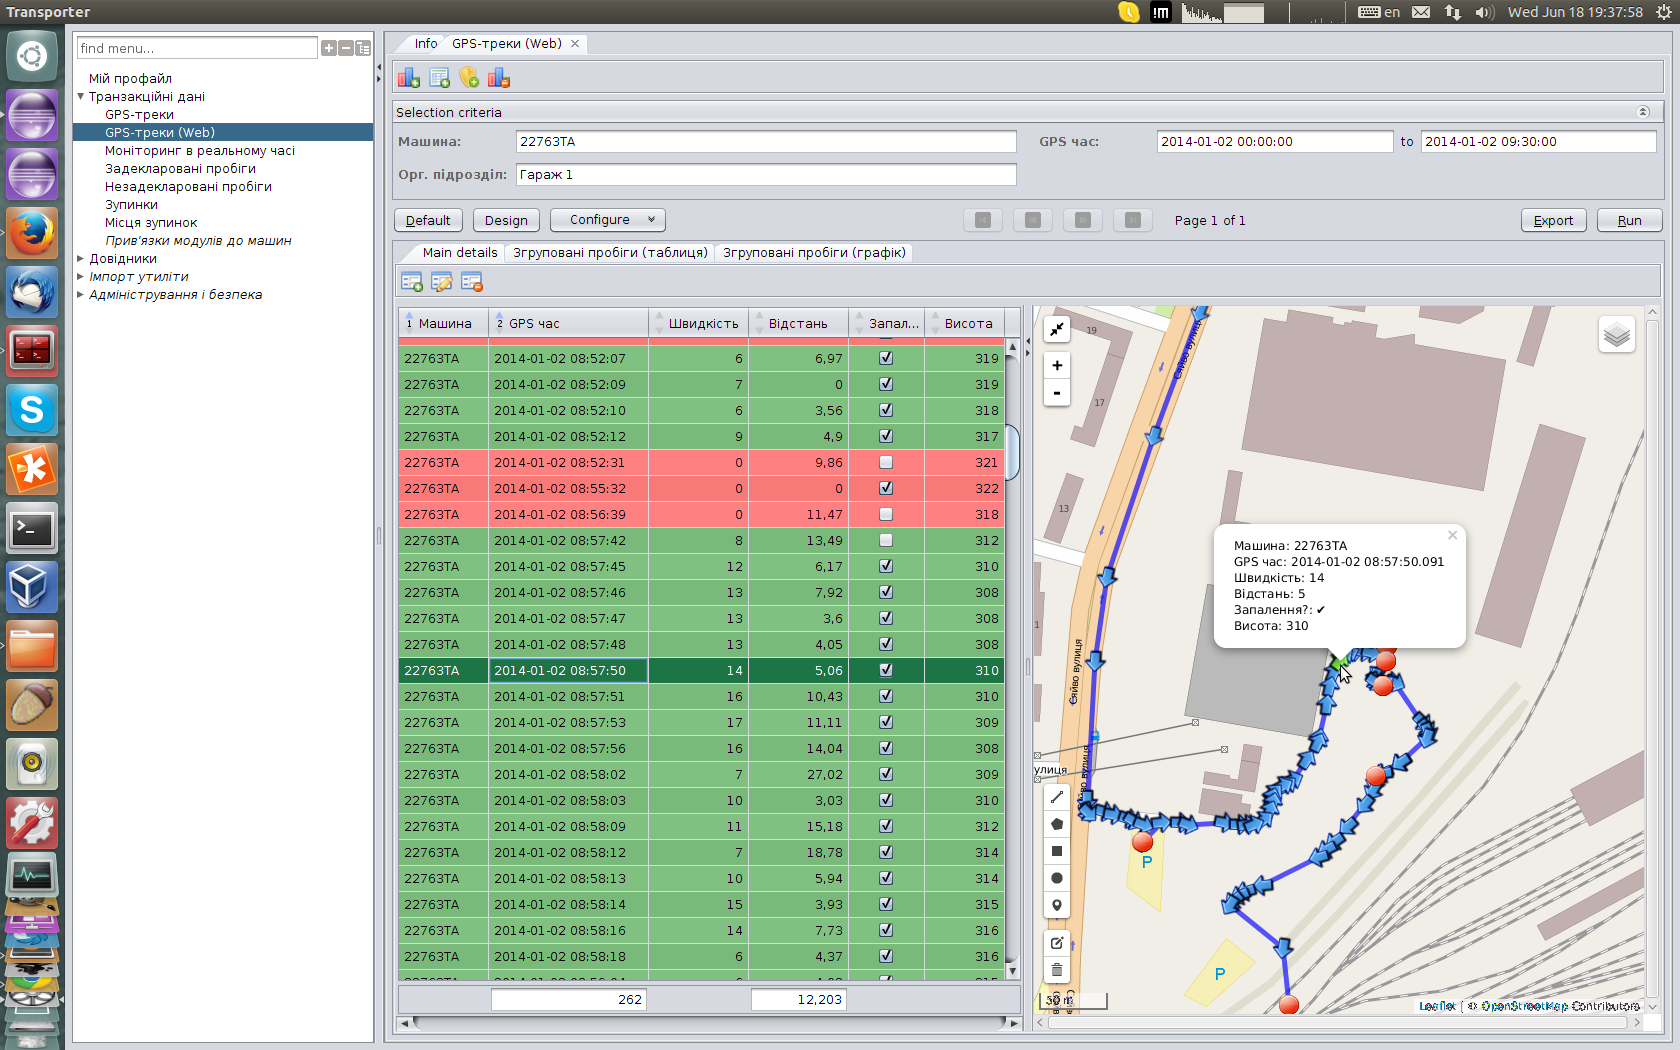
\includegraphics[width=16cm]{chapters/02-gpstracks/images/16-selected-message-with-popup.png}
\caption{selected-message-with-popup}\label{fig:16}
\end{figure}

\begin{figure}[!htp]
\centering
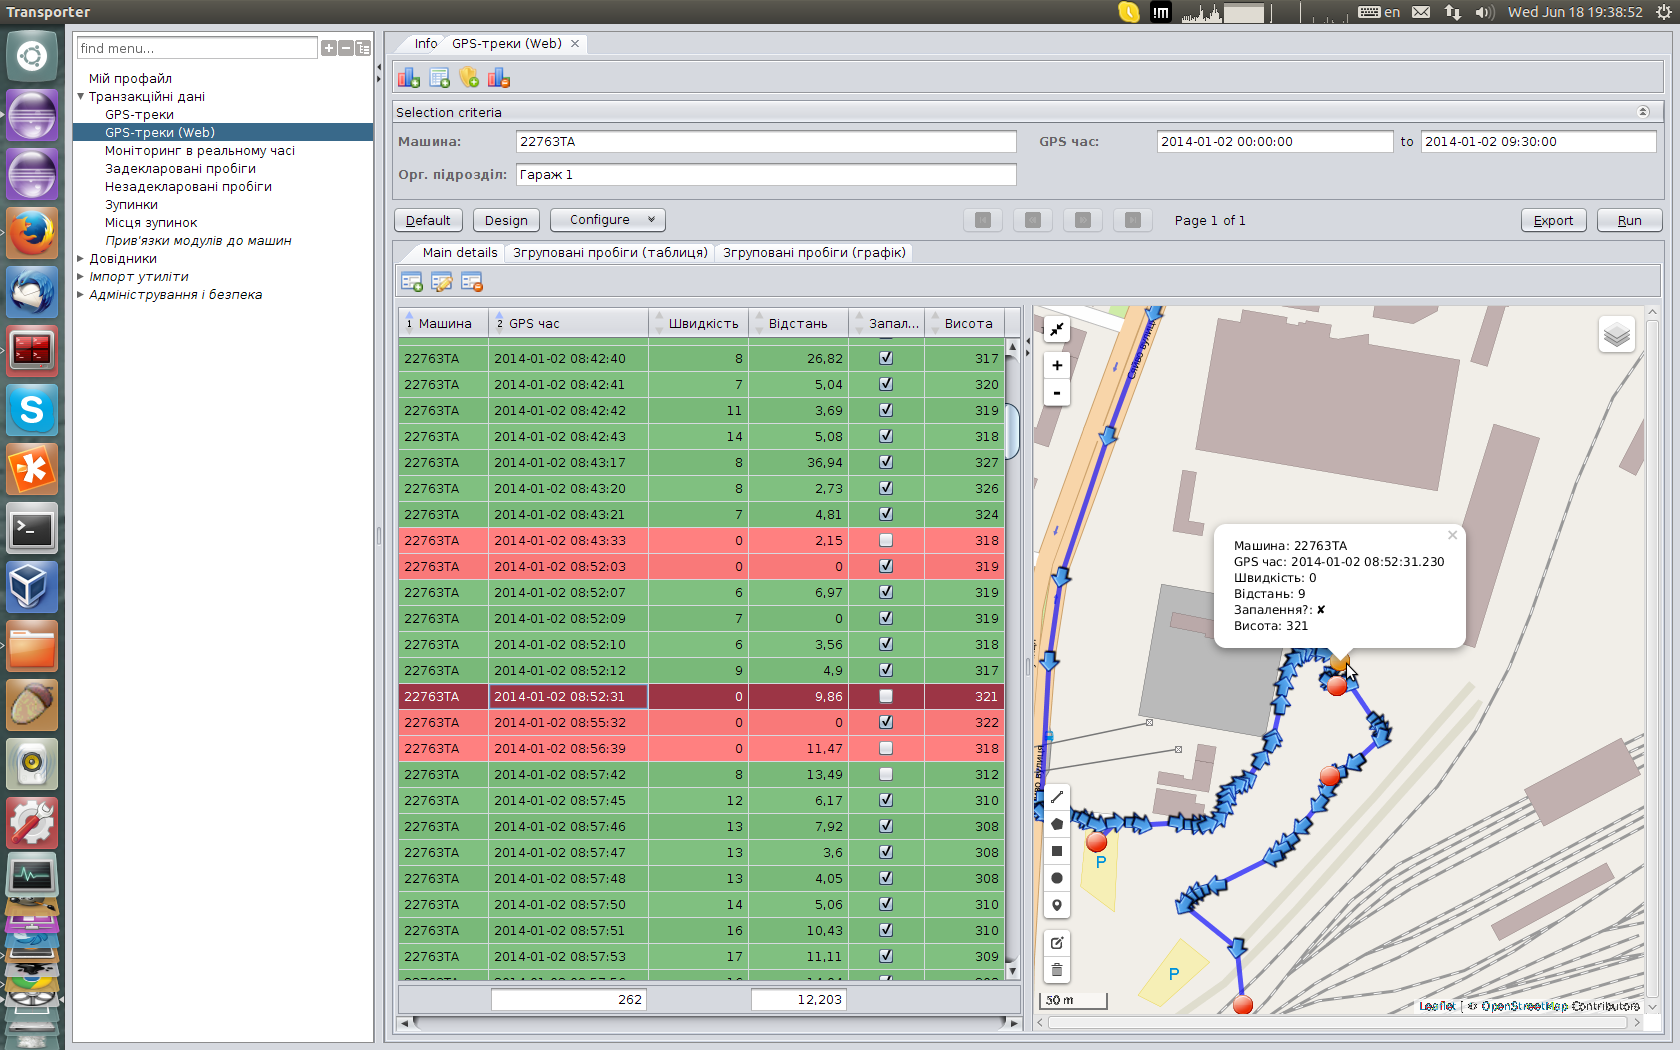
\includegraphics[width=16cm]{chapters/02-gpstracks/images/17-selected-stoppage-with-popup.png}
\caption{selected-stoppage-with-popup}\label{fig:17}
\end{figure}

\begin{figure}[!htp]
\centering
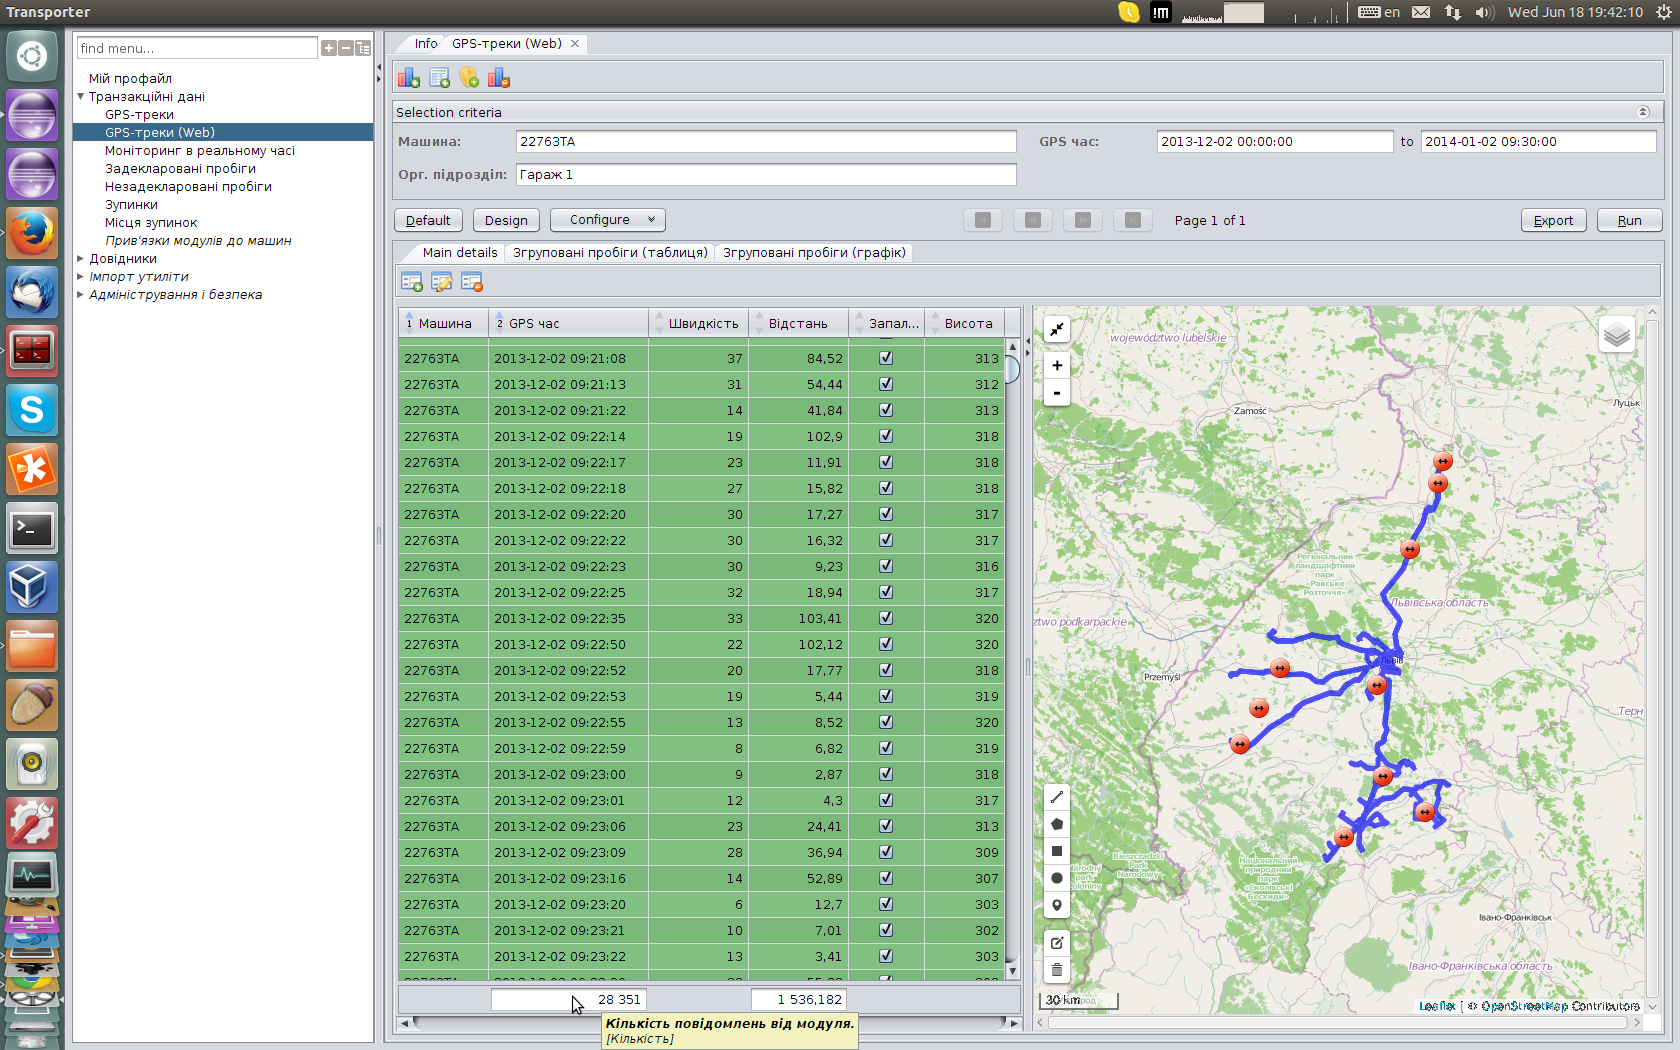
\includegraphics[width=16cm]{chapters/02-gpstracks/images/18-huge-dataset-processed-1machine-1month.png}
\caption{huge-dataset-processed-1machine-1month}\label{fig:18}
\end{figure}

\begin{figure}[!htp]
\centering
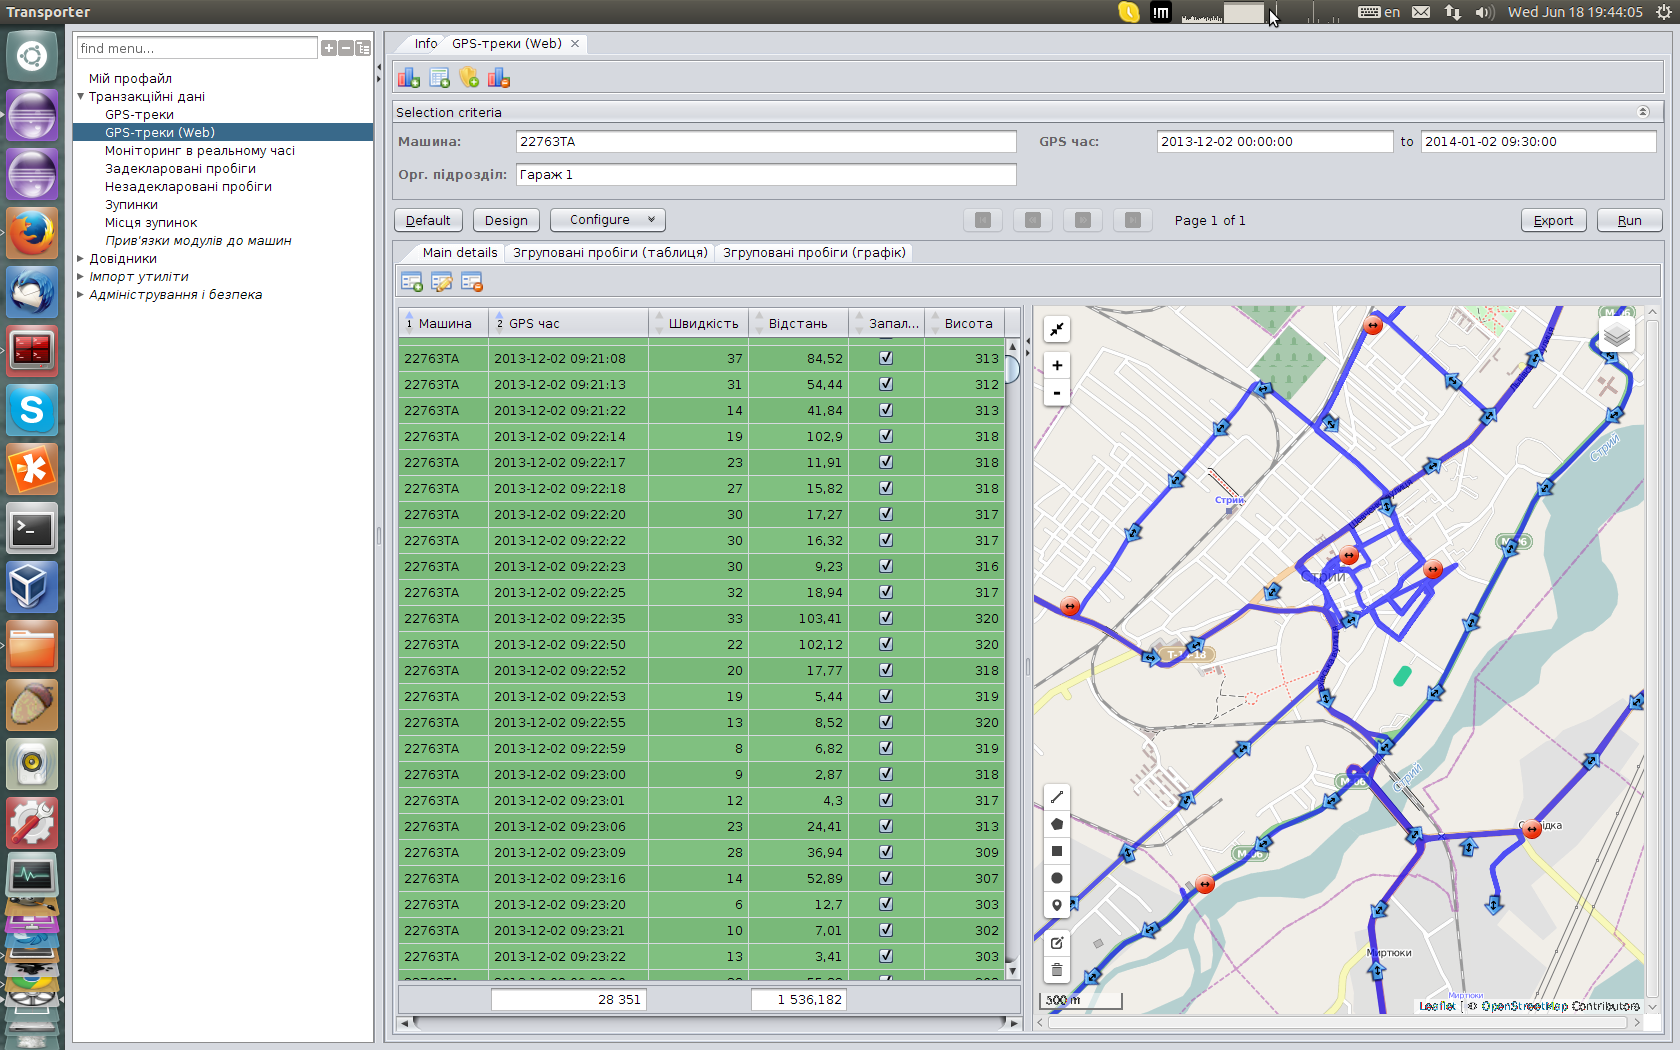
\includegraphics[width=16cm]{chapters/02-gpstracks/images/19-middle-details-at-some-place.png}
\caption{middle-details-at-some-place}\label{fig:19}
\end{figure}

\begin{figure}[!htp]
\centering
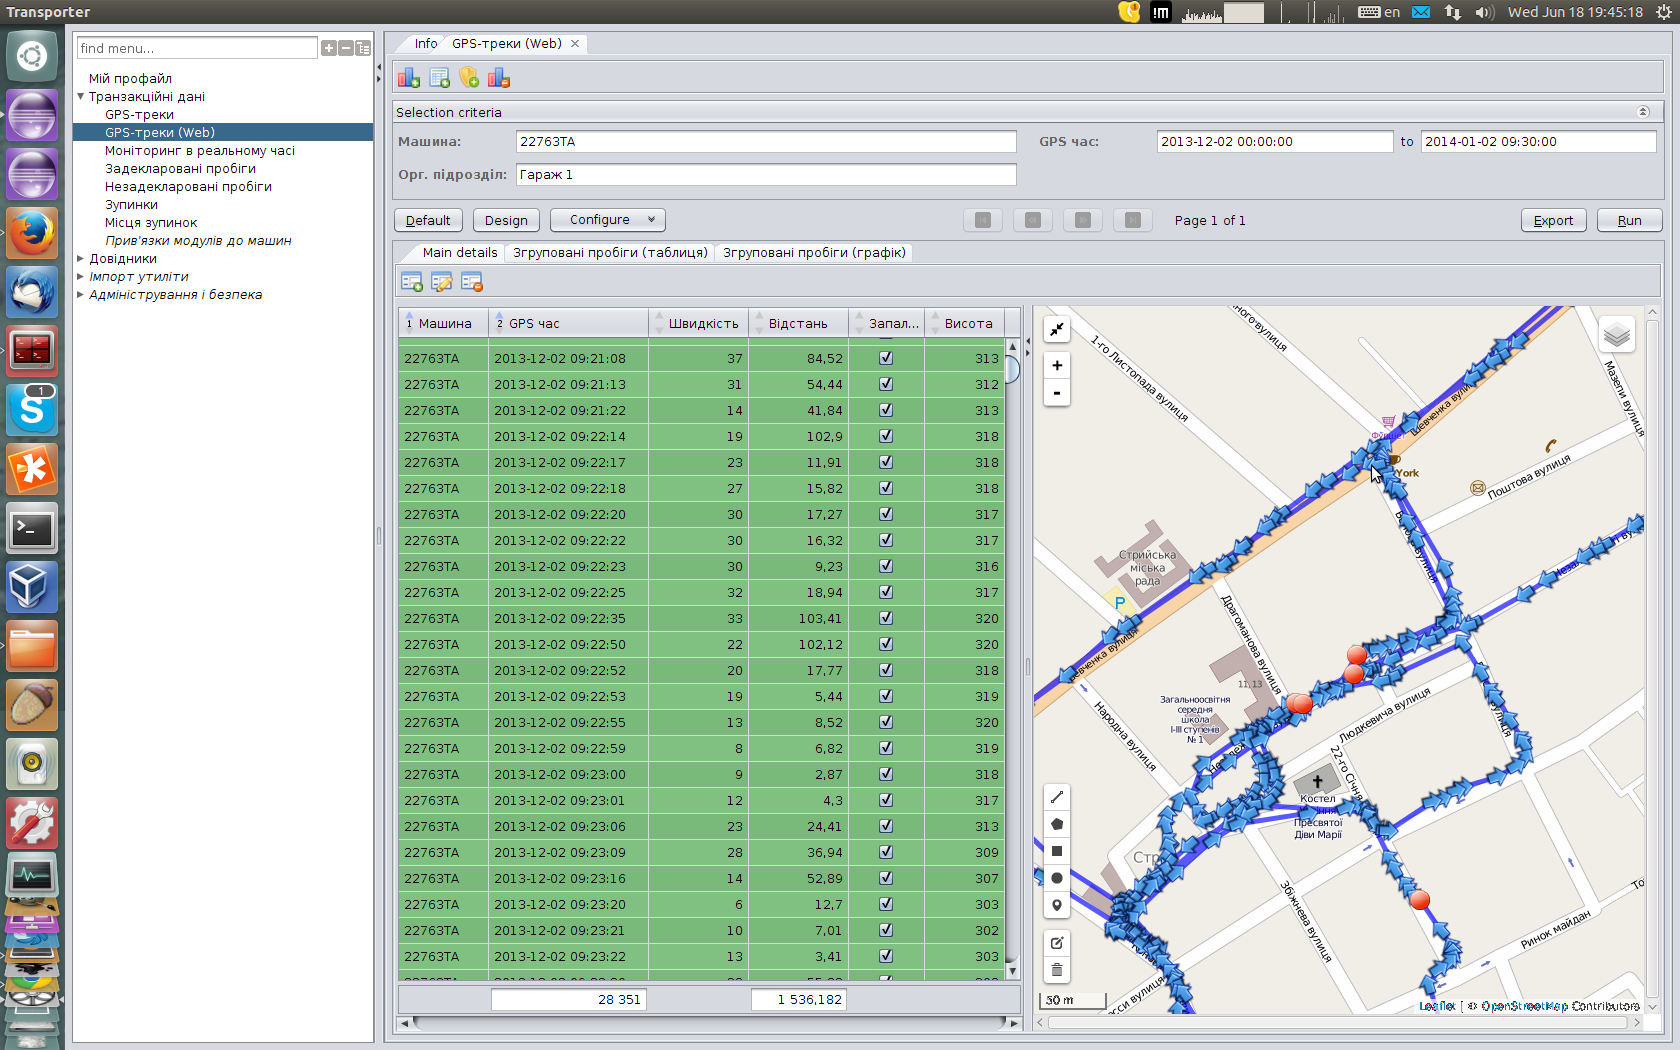
\includegraphics[width=16cm]{chapters/02-gpstracks/images/20-full-details-and-marker-hovering-feature.png}
\caption{full-details-and-marker-hovering-feature}\label{fig:20}
\end{figure}